\chapter{Definición del Problema}

\section{Producto Rápido de Enteros}
Para entender los métodos para el producto rápido de enteros, debemos definir la cota inicial con la cual se compararan aquellos métodos que se consideran \textit{rápidos} por sobre lo habitual. Comenzamos definiendo el \textit{naive method}~\cite{Heideman1985} que se utiliza al momento de considerar un producto entre números.\\

Una forma de definir la complejidad de este método es trabajando con polinomios, luego consideramos dos números enteros no-negativos $a,b$, reescritos como polinomios, de modo que la multiplicación entre ellos se expresa como:\\

\begin{align}
\begin{split}
    a(x) &= \sum_{j=0}^{\frac{n}{2}-1}{a_{j}x^{j}} = a_{0} + a_{1}x + ... + a_{\frac{n}{2}-1}x^{\frac{n}{2}-1}\\
    b(x) &= \sum_{j=0}^{\frac{n}{2}-1}{b_{j}x^{j}} = b_{0} + b_{1}x + ... +b_{\frac{n}{2}-1}x^{\frac{n}{2}-1}\\
    c(x) &= a(x)b(x) = \left(\sum_{j=0}^{\frac{n}{2}-1}{a_{j}x^{j}}\right) \left(\sum_{j=0}^{\frac{n}{2}-1}{b_{j}x^{j}}\right),
\end{split}\label{poliClassic}
\end{align}\\
esta operación nos lleva a realizar $n^2$ multiplicaciones y $(n-1)^2$ sumas, obteniendo una complejidad final de $O(n^2)$.\\

A partir de esto, los métodos para el producto rápido de enteros serán aquellos que logren cotas inferiores a $O(n^2)$.

\subsection{Método de Karatsuba}
Sean dos números enteros no-negativos $a,b$ con base $B$, almacenados como arreglos del tipo $a_{0},a_{1},a_{2},...,a_{n-1}$ y de largo $n$, tal que $a=\sum^{n-1}_{i=0}{a_{i}\cdot B^{i}}$, y de forma análoga para el número $b$.\\

Aplicando un método clásico de \textit{divide and conquer}, podemos dividir los números en dos mitades, obteniendo la siguiente representación:
\begin{align}
\begin{split}
    a &= a_{H}B^{m}+a_{L}\\
    b &= b_{H}B^{m}+b_{L},
\end{split}\label{divkar::1}
\end{align}
donde $m=\lceil\frac{n}{2}\rceil$ y el sub-índice $H$ indica la parte alta de la división y $L$ la parte baja, tal que $a_{L}=\sum^{m-1}_{i=0}{a_{i}\cdot B^{i}}$ y $a_{H}=\sum^{m-1}_{i=0}{a_{i+m}\cdot B^{i}}$, y de forma análoga para $b$.\\

Luego el producto $ab$ se puede expresarse de forma \textit{naive} como:
\begin{align}
\begin{split}
    ab &= (a_{H}B^{m}+a_{L})(b_{H}B^{m}+b_{L})\\
    &= a_{H}b_{H}B^{2m} + (a_{H}b_{L} + a_{L}b_{H})B^{m} + a_{L}b_{L}.
\end{split}\label{divkar::2}
\end{align}
Dado que se trata de una ecuación diseñada con una técnica de \textit{divide and conquer}, es posible utilizar el Teorema Maestro~\cite{10.1145/1008861.1008865} para calcular su complejidad, obteniendo la ecuación asintótica $T(n)=4T(\frac{n}{2}) + O(n)$, equivalente a una cota de $O(n^2)$. Este caso, (\ref{divkar::2}) debe tener la misma complejidad que (\ref{poliClassic}), dado que ambos son \textit{naive methods}.\\

El método propuesto por \textit{Karatsuba et al.}~\cite{Karatsuba1962} aplica el mismo mecanismo descrito anteriormente de división de los números $a,b$, pero considerado el siguiente cambio de variables~\cite{luders2015fast}:
\begin{align}
\begin{split}
    u &= a_{H}b_{H}\\
    v &= (a_{H} - a_{L})(b_{H} - b_{L})\\
    w &= a_{L}b_{L}.
\end{split}\label{divkar::3}
\end{align}

Luego, el producto $ab$ queda reescrito~\cite{luders2015fast} como:
\begin{align}
\begin{split}
    ab=& u\left(1+B^{m}\right)-v B^{m}+w\left(B^{m}+B^{2m}\right) \\
    =& a_{L} b_{L}\left(1+B^{m}\right)-\left(a_{L}-a_{H}\right)\left(b_{L}-b_{H}\right) B^{m}+a_{H} b_{H}\left(B^{m}+B^{2m}\right) \\
    =& a_{L} b_{L}+a_{L} b_{L} B^{m}-a_{L} b_{L} B^{m}+a_{L} b_{H} B^{m}+a_{H} b_{L} B^{m}-a_{H} b_{H} B^{m}+\\
& a_{H} b_{H} B^{m}+a_{H} b_{H} B^{2m} \\
    =& a_{L} b_{L}+\left(a_{L} b_{H}+a_{H} b_{L}\right) B^{m}+a_{H} b_{H} B^{2 m},
\end{split}\label{divkar::4}
\end{align}
de este modo, la ecuación asintótica resultante es $T(n)=3T(\frac{n}{2}) + O(n)$, obteniendo una cota de $O(n^{\log_{2}{3}})\approx O(n^{1.585})$ para el método de \textit{Karatsuba}.

\subsection{Métodos de Toom-Cook}

Siguiendo la lógica de implementar la técnica de \textit{divide and conquer} que utiliza \textit{Karatsuba} para fragmentar un producto, la familia de métodos de \textit{Toom-Cook} es un conjunto infinito de algoritmos que generalizan la división de factores de un producto de polinomios. Fue desarrollado gracias al trabajo de \textit{Toom}~\cite{Toom1963TheCO} y \textit{Cook}~\cite{10.2307/1995359} y su aplicación se denomina como \textit{Toom-Cook k}; el caso de \textit{Toom-Cook 2} corresponde al método de \textit{Karatsuba}.\\

De acuerdo al trabajo de \textit{Zanoni} en ~\cite{10.1145/1837934.1837995}, es posible generalizar el conjunto de métodos en 5 etapas: \textbf{Splittinng}, \textbf{Evaluation}, \textbf{Recursion}, \textbf{Interpolation} y \textbf{Recomposition}.
Consideremos dos números enteros no-negativos $u,v$, tal que buscamos el producto $w=uv$ de acuerdo a las etapas anteriormente descrita.

\paragraph{Splittinng}
Sean dos números enteros no-negativos $a,b$ con base $B$, expresados como polinomios de grados $d_{1}$, $d_{2}$ respectivamente, descritos como:
\begin{equation}
    a(x,h)=\sum^{d_{1}}_{i=0}{a_{i}x^{i}h^{d_{1}-i}} \quad ; \quad b(x,h)=\sum^{d_{2}}_{i=0}{b_{i}x^{i}h^{d_{2}-i}}.
\end{equation}
En este caso, $u=a(B,1)$ y $v=b(B,1)$, luego buscamos el producto $c(x,h)=a(x,h)b(x,h)$, con $deg(c)=d_{1}+d_{2}$. En la general $d_{1}=d_{2}=k-1$ para \textit{Toom-Cook k}.


\paragraph{Evaluation}
Seleccionar $2k-1$ valores $v_{i}=(v_{i}',v_{i}'')$ con $v_{i}'$ y $v_{i}''$ coprimos entre ellos y tal que $v_{i} \neq \pm v_{j}$ para $j \neq i$; evaluar cada operando, obteniendo $a(v_{i})$ y $b(v_{i})$.

\paragraph{Recursion}
Calcular el factor $w_{i}=a(v_{i})b(v_{i})$ de manera recursiva. Luego, se define el vector $\vec{w}=(w_{i})$.

\paragraph{Interpolation}
Resolver el problema de interpolación $c(v_{i})=w_{i}$ invirtiendo la matriz pseudo-Vandermonde $A_{k}$ generada por los valores $v_{i}$, tal que $\vec{c}=A^{-1}_{k}\vec{w}$, donde $\vec{c}=(c_{i})$ es el vector de coeficientes de $c(x,h)$.

\paragraph{Recomposition}
Una vez computado todos los coeficientes, es posible evaluar $w=c(B,1)$.\\

De manera general, la complejidad de los métodos \textit{Toom-Cook k} viene dada por $O(n^{\log_{k}{(2k-1)}})$.

\subsection{Método de Schonhage Strassen}
El método de \textit{Schonhage Strassen}~\cite{SchonhageS71} puede ser implementado por medio del  \textit{Teorema de la Convolución} y la \textit{Trasformada Rápida de Fourier}, donde el primer algoritmo utiliza la \textit{Trasformada Discreta de Fourier} sobre aproximaciones finitas en $\C$, mientras que el segundo algoritmo utiliza la misma idea que el primero pero sobre el espacio finitos de anillos $\Z_{2^{2n}-1}$ en lugar de $\C$.

\subsubsection{Schonhage Strassen - Aproximación en $\C$}
Sea $x$ un número entero no-negativo con base $B$ representado como el vector $x\in\Z^{n}_{B}=\{0,1,2,...,B-1\}^{n}$ y descrito como:
\begin{equation}
    x=\sum^{n-1}_{i=0}{x_{i}B^{i}}.
\end{equation}

\paragraph{Trasformada Discreta de Fourier (DFT)}
La \textit{DFT} es una transformación de $\C^{n}$ a $\C^{n}$, tal que $\hat{x}\in\C^{n}$ es la \textit{DFT} de $x\in\C^{n}$, definida como:
\begin{equation}
    \hat{x}_{i}=\sum^{n-1}_{j=0}{x_{j}\omega^{ij}} \quad \text{con} \quad (0\leq i\leq n-1),
\end{equation}
con $\omega=\exp^{\frac{2\pi i}{n}}$.

\subparagraph{Lema 1}Sea $n>1$ y $\omega=\exp{\frac{2\pi i}{n}}$ se tiene que:
\begin{equation}
    \omega^{n}=1 \text{ y } \omega^{k} \neq 1 \text{ para todo } 0<k<n
\end{equation}
y para todo $0<k<n$ se tiene:
\begin{equation}
    \sum^{n-1}_{i=0}{\omega^{ik}}=0
\end{equation}

Luego, asumiendo \textit{DFT} una función biyectiva y por ende con inversa igual a $\Check{x}$ y definida:
\begin{equation}
    \Check{x}_{i} = \frac{1}{n}\sum^{n-1}_{j=1}{x_{j}\omega^{-ij}} \quad \text{con} \quad (0\leq i\leq n-1),
\end{equation}
se tiene que su evaluación rápida viene dada por la siguiente definición de \textit{Cooley-Tukey}~\cite{Cooley1965AnAF}.

\paragraph{Trasformada Rápida de Fourier (FFT)}
Sea $n$ una potencia de 2 y $x\in\C^{n}$, utilizando una estrategia \textit{divide and conquer}, se definen las partes $x_{par},x_{impar}\in\C^{\frac{n}{2}}$ como:
\begin{equation}
    (x_{par})_{i} = x_{2i} \quad (x_{impar})_{i} = x_{2i+1},
\end{equation}
para todo $i$ con $0\leq i \leq \frac{n}{2}-1$. Una visualización de esta estrategia se encuentre en la Figura \ref{fig:intro:fft:tree}.\\

\begin{figure}[H]
    \centering
    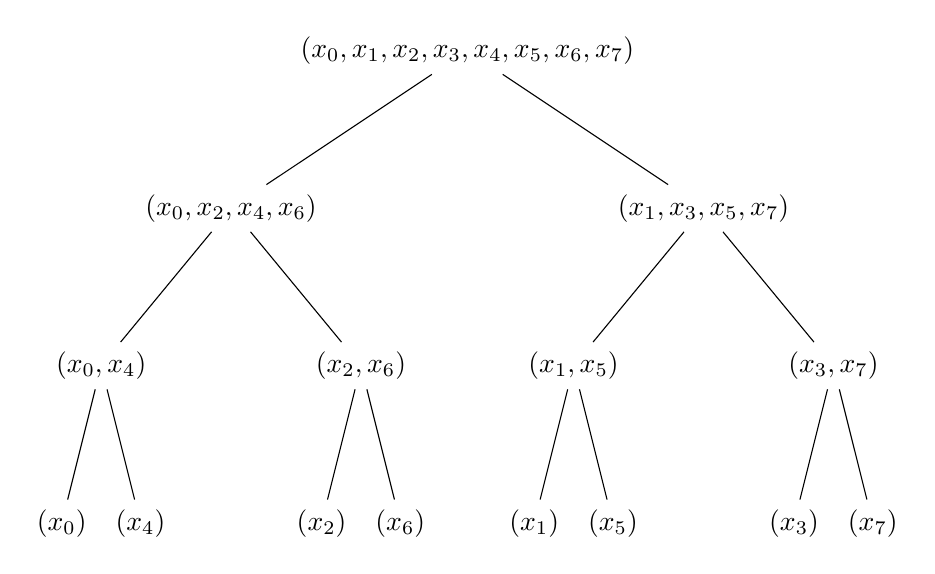
\begin{tikzpicture}[level distance=2cm]
    
    \tikzstyle{level 1}=[sibling distance=60mm]
    \tikzstyle{level 2}=[sibling distance=33mm]
    \tikzstyle{level 3}=[sibling distance=10mm]
    \tikzstyle{level 4}=[sibling distance=5mm]
    
    \node (Root) {$(x_{0},x_{1},x_{2},x_{3},x_{4},x_{5},x_{6},x_{7})$}
    child {
        node {$(x_{0},x_{2},x_{4},x_{6})$}
        %child { node {4} edge from parent node[left,draw=none] {help!} }
        child { 
            node {$(x_{0},x_{4})$} 
                child { 
                    node {$(x_{0})$}
                }
                child { 
                    node {$(x_{4})$}
                }
        }
        child { 
            node {$(x_{2},x_{6})$} 
                child { 
                    node {$(x_{2})$}
                }
                child { 
                    node {$(x_{6})$}
                }
        }
    }
    child {
        node {$(x_{1},x_{3},x_{5},x_{7})$}
        child { 
            node {$(x_{1},x_{5})$} 
                child { 
                    node {$(x_{1})$}
                }
                child { 
                    node {$(x_{5})$}
                }
        }
        child { 
            node {$(x_{3},x_{7})$} 
            child { 
                    node {$(x_{3})$}
                }
            child { 
                node {$(x_{7})$}
            }
        }
    };
    \end{tikzpicture}
    
    \caption{Visualización de la estrategia \textit{divide and conquer} utilizada en \textit{FFT}. Figura modifica desde \cite{luders2015fast}.}
    \label{fig:intro:fft:tree}
\end{figure}

Finalmente, la \textit{FFT} de $x\in\C^{n}$ se define como:
\begin{align}
    \hat{x}_{i} &= \sum^{n-1}_{j=0}{x_{j}\omega^{ij}}\\
    &= \sum^{n/2 -1}_{j=0}{(x_{par})_{j}(\omega^{2})^{ij}} + \omega^{i}\sum^{n/2 -1}_{j=0}{(x_{impar})_{j}(\omega^{2})^{ij}}\\
    &= (\hat{x}_{par})_{i\;\mathrm{mod}\; n/2} + \omega^{i}(\hat{x}_{impar})_{i\;\mathrm{mod}\; n/2}.
\end{align}
Notar que tanto $\hat{x}_{par}$ como $\hat{x}_{impar}$ se calculan de manera recursiva.

\paragraph{Teorema de la Convolución} Antes de definir la implementación del método de \textit{Schonhage-Strassen}, es necesario desarrollar la teoría del operador que se utilizará, la convolución.\\

Sean $u,v\in\C^{n}$ interpretados como los coeficientes de dos polinomios tales como:
\begin{align}
\begin{split}
    f_{u}(z) &= u_{0} + u_{1}z, u_{2}z^{2}, ... , u_{n-1}z^{n-1}\\
    f_{v}(z) &= v_{0} + v_{1}z, v_{2}z^{2}, ... , v_{n-1}z^{n-1},
\end{split}\label{conv:1}
\end{align}
se define el operador de convolución, $u*b$ como el vector de coeficientes obtenido al multiplicar los polinomios de la forma $f_{u}$ y $f_{v}$. En tal caso, el factor resultante será $f_{u*v}(z)=f_{u}(z)f_{v}(z)$ para todo $z\in\C$.\\

Formalmente, el teorema de la convolución se define para $u,v\in\C^{n}$ y $w=u*v\in\C^{m}$, con $m=2n-1$, y tal que:
\begin{align*}
    u' &= (u_{0},u_{1},...,u_{n-1},0,...,0)\\
    v' &= (v_{0},v_{1},...,v_{n-1},0,...,0)
\end{align*}
donde la cantidad de ceros corresponderá a los factores faltantes para completar la dimensión en $C^{m}$, luego, para todo $i$ con $0\leq i \leq m-1$ tal que:
\begin{equation}
    \hat{w}_{i} = \hat{u}'_{i}\hat{v}'_{i}
\end{equation}
con $\hat{x}$ la aplicación de la \textit{FFT} sobre $x$, con $O(n\log(n))$ operaciones.


\paragraph{Implementación Schonhage-Strassen}
Sean $a,b$ dos números enteros no-negativo con base $B$, y con la misma representación que (\ref{conv:1}), tal que $a=f_{a}(B)$ y $b=f_{b}(B)$; el método de \textit{Schonhage-Strassen} define el producto $ab$ como:
\begin{equation}
    ab = f_{a}(B)f_{b}(B) = f_{a*b}(B).
\end{equation}

El algoritmo primero calcula la convolución $a*b$ para luego evaluar $f_{a*b}(B)$. Esta implementación del método de \textit{Schonhage-Strassen}  considera $O(n\log(n))$~\cite{DBLP:journals/corr/abs-1006-0405} operaciones.

%\subsubsection{Schonhage Strassen - Aproximación en Anillos}

%\subsection{Método de Fürer}